\section{Validación comercial inicial y diseño del piloto}

\subsection{Ficha técnica de la encuesta}

La encuesta se aplicó mediante Google Forms entre el 8 y el 24 de julio de 2026
\parencite{encuesta_gymhub_2026}.
Se consultó a personas adultas vinculadas a gimnasios a las que el equipo pudo
acceder. Esta selección se conoce como muestreo por conveniencia. Los
resultados se usan para orientar el proyecto dentro de los límites de esa
muestra. Las 15 personas
participaron voluntariamente, aceptaron el consentimiento inicial y no
proporcionaron nombres, correos ni datos de salud.

La muestra quedó compuesta por tres dueños o administradores, dos entrenadores
con responsabilidades administrativas y diez miembros. Se alcanzó la meta de
miembros, mientras que el acceso a responsables fue más difícil porque varios
dueños rechazaron participar. Las cinco respuestas administrativas obtenidas se
utilizan como información descriptiva para orientar el piloto.

\begin{figure}[htbp]
\centering
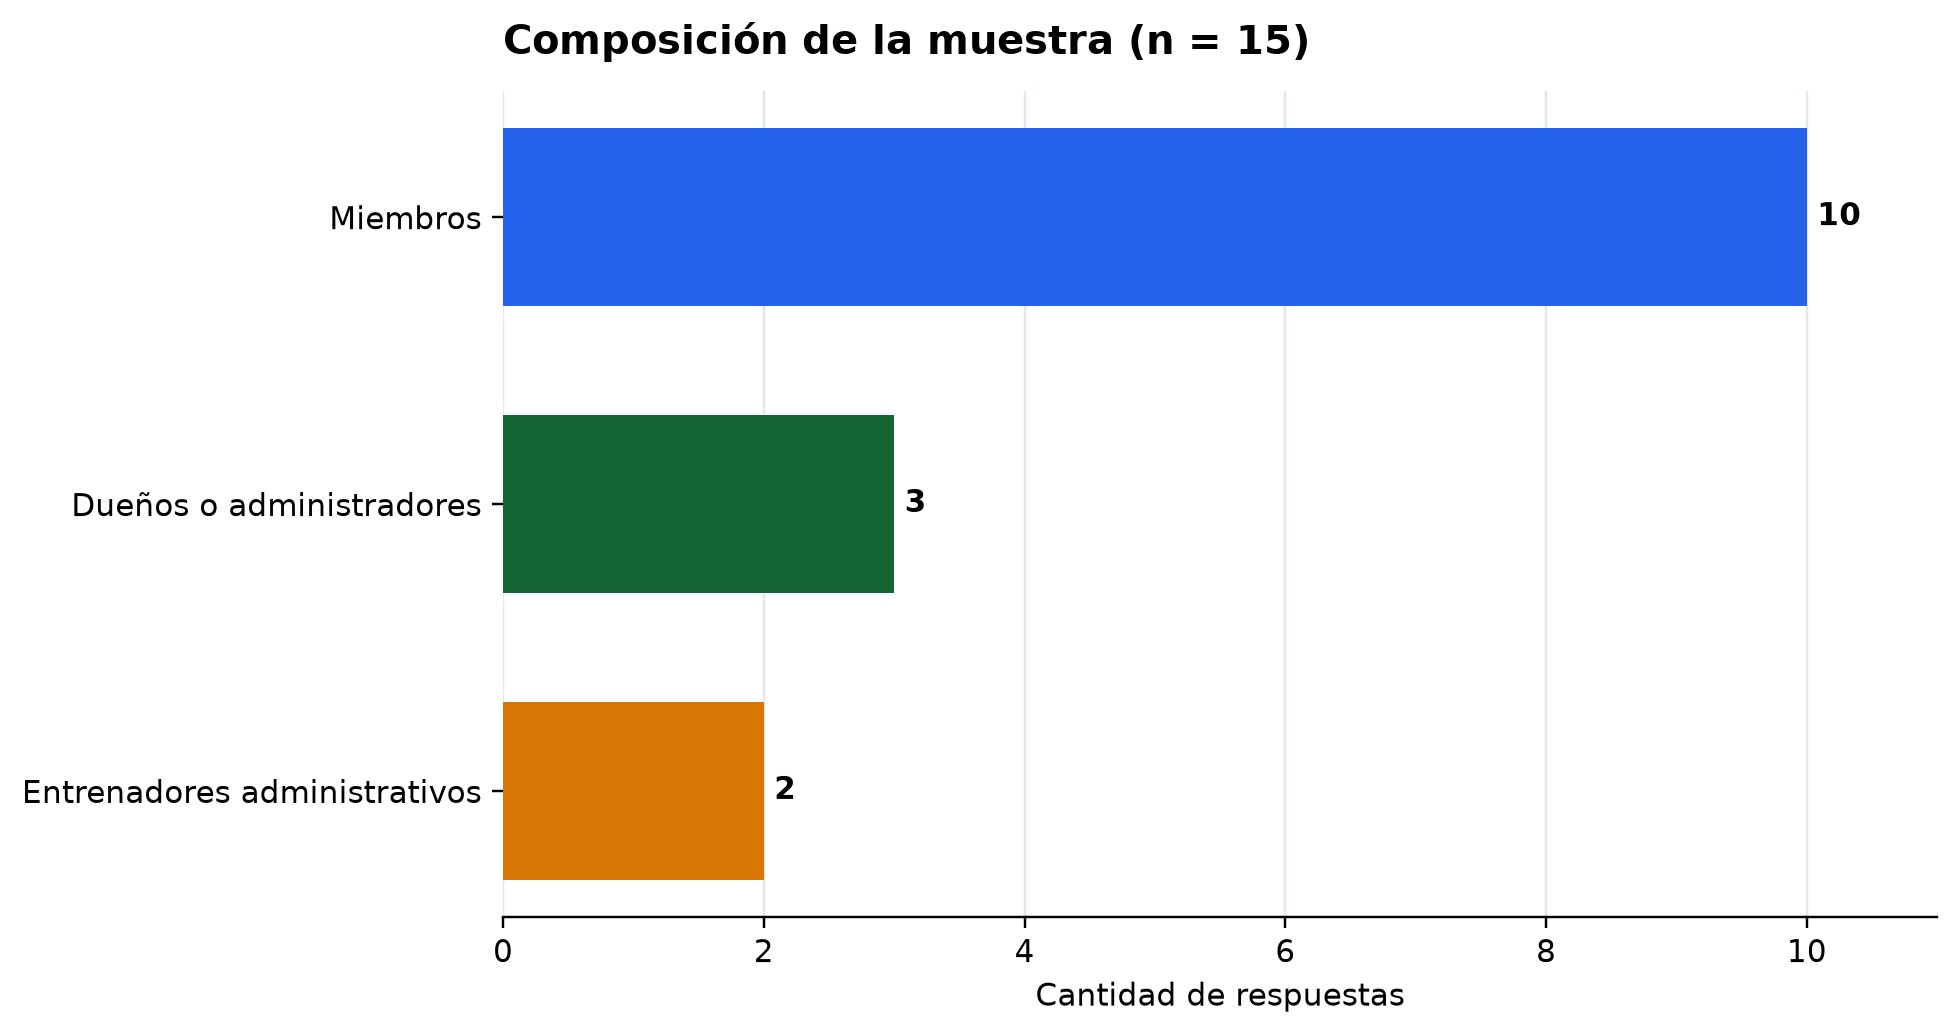
\includegraphics[width=0.88\textwidth]{imagenes/encuesta_composicion_muestra.png}
\caption{Composición de la muestra de validación}
\label{fig:encuesta-muestra}
\caption*{\textit{Nota}. Elaboración propia a partir de 15 respuestas válidas \parencite{encuesta_gymhub_2026}.}
\end{figure}

\subsection{Resultados de responsables}

Los cinco responsables ubicaron el gimnasio relacionado en Pérez Zeledón. Dos
indicaron administrar entre 76 y 150 miembros, uno más de 150 y dos no conocían
el tamaño. Las herramientas utilizadas no fueron excluyentes: papel, hojas de
cálculo, software especializado y sistemas internos obtuvieron dos menciones
cada uno; WhatsApp obtuvo una.

El cobro y los pagos pendientes fueron la dificultad más frecuente, con cuatro
menciones. Entre las funciones valoradas, membresías, asistencia, planes de
entrenamiento, sesiones y progreso, y alertas o reportes obtuvieron dos menciones
cada una. Las respuestas se conservaron tal como fueron recolectadas; la oferta
actual prioriza cobros, planes, asistencia y seguimiento, no todos los elementos
consultados. Tres responsables prefieren una combinación de dispositivos, uno
computadora y uno celular. Los cinco calificaron el control de acceso como
importante o muy importante.

\begin{figure}[htbp]
\centering
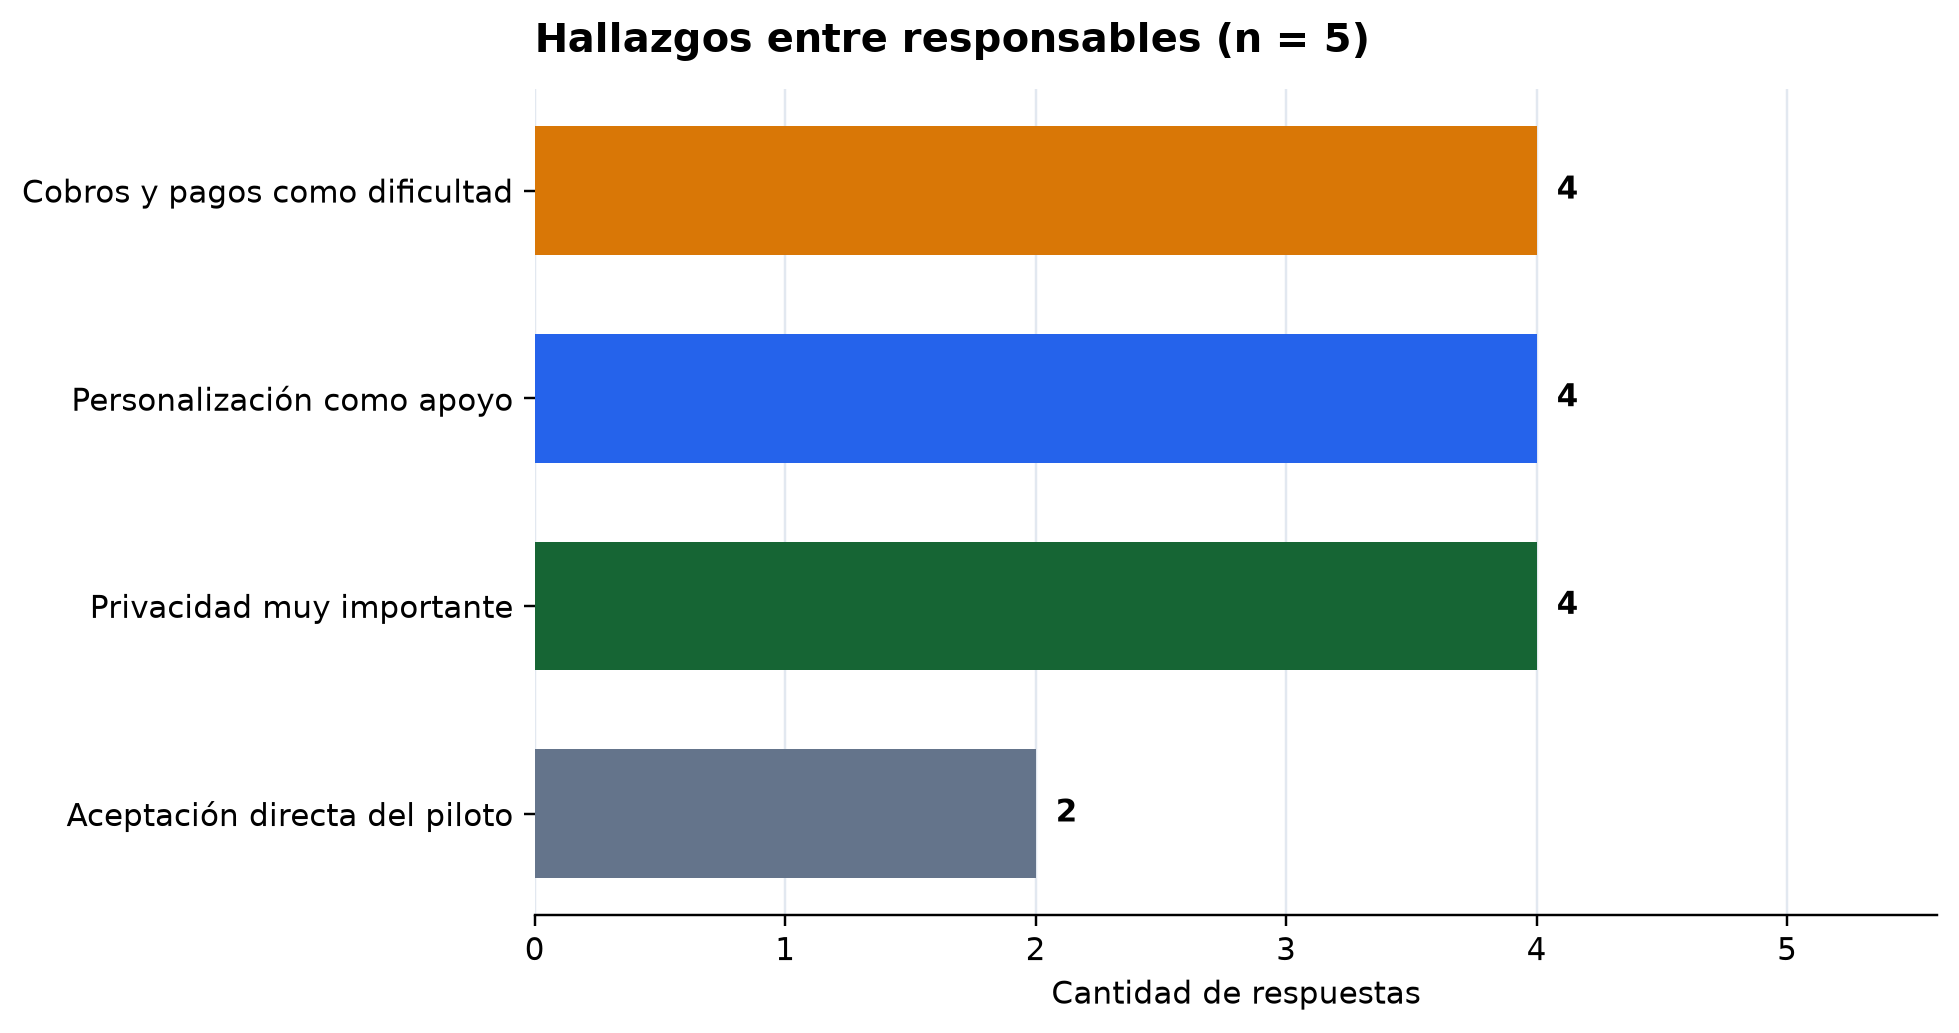
\includegraphics[width=0.9\textwidth]{imagenes/encuesta_resultados_responsables.png}
\caption{Hallazgos de responsables de gimnasios}
\label{fig:encuesta-responsables}
\caption*{\textit{Nota}. Al tratarse de preguntas de selección múltiple, las cantidades no corresponden a categorías excluyentes. Elaboración propia a partir de la encuesta \parencite{encuesta_gymhub_2026}.}
\end{figure}

Dos responsables aceptaron directamente probar la plataforma durante cuatro
semanas, uno respondió que dependería de las condiciones, uno indicó tal vez y
uno respondió que no. En cuatro de los cinco casos hubo interés o posibilidad
de probarla. Además, cuatro solicitaron una demostración antes de indicar un
precio y la única respuesta monetaria se ubicó entre CRC 7\,500 y CRC 15\,000.
Por ello se diseñó un piloto de CRC 15\,000 que permite conocer Pulso antes de
seleccionar un plan regular. Starter, por CRC 15\,000, y Pro Gym, por
CRC 25\,000, son precios propuestos que aún deben probarse con posibles
clientes. En el proceso de planificación se habían considerado planes de
CRC 30\,000, CRC 45\,000 y CRC 60\,000; esa combinación se reemplazó por
la propuesta comercial presentada en este informe.

\begin{figure}[htbp]
\centering
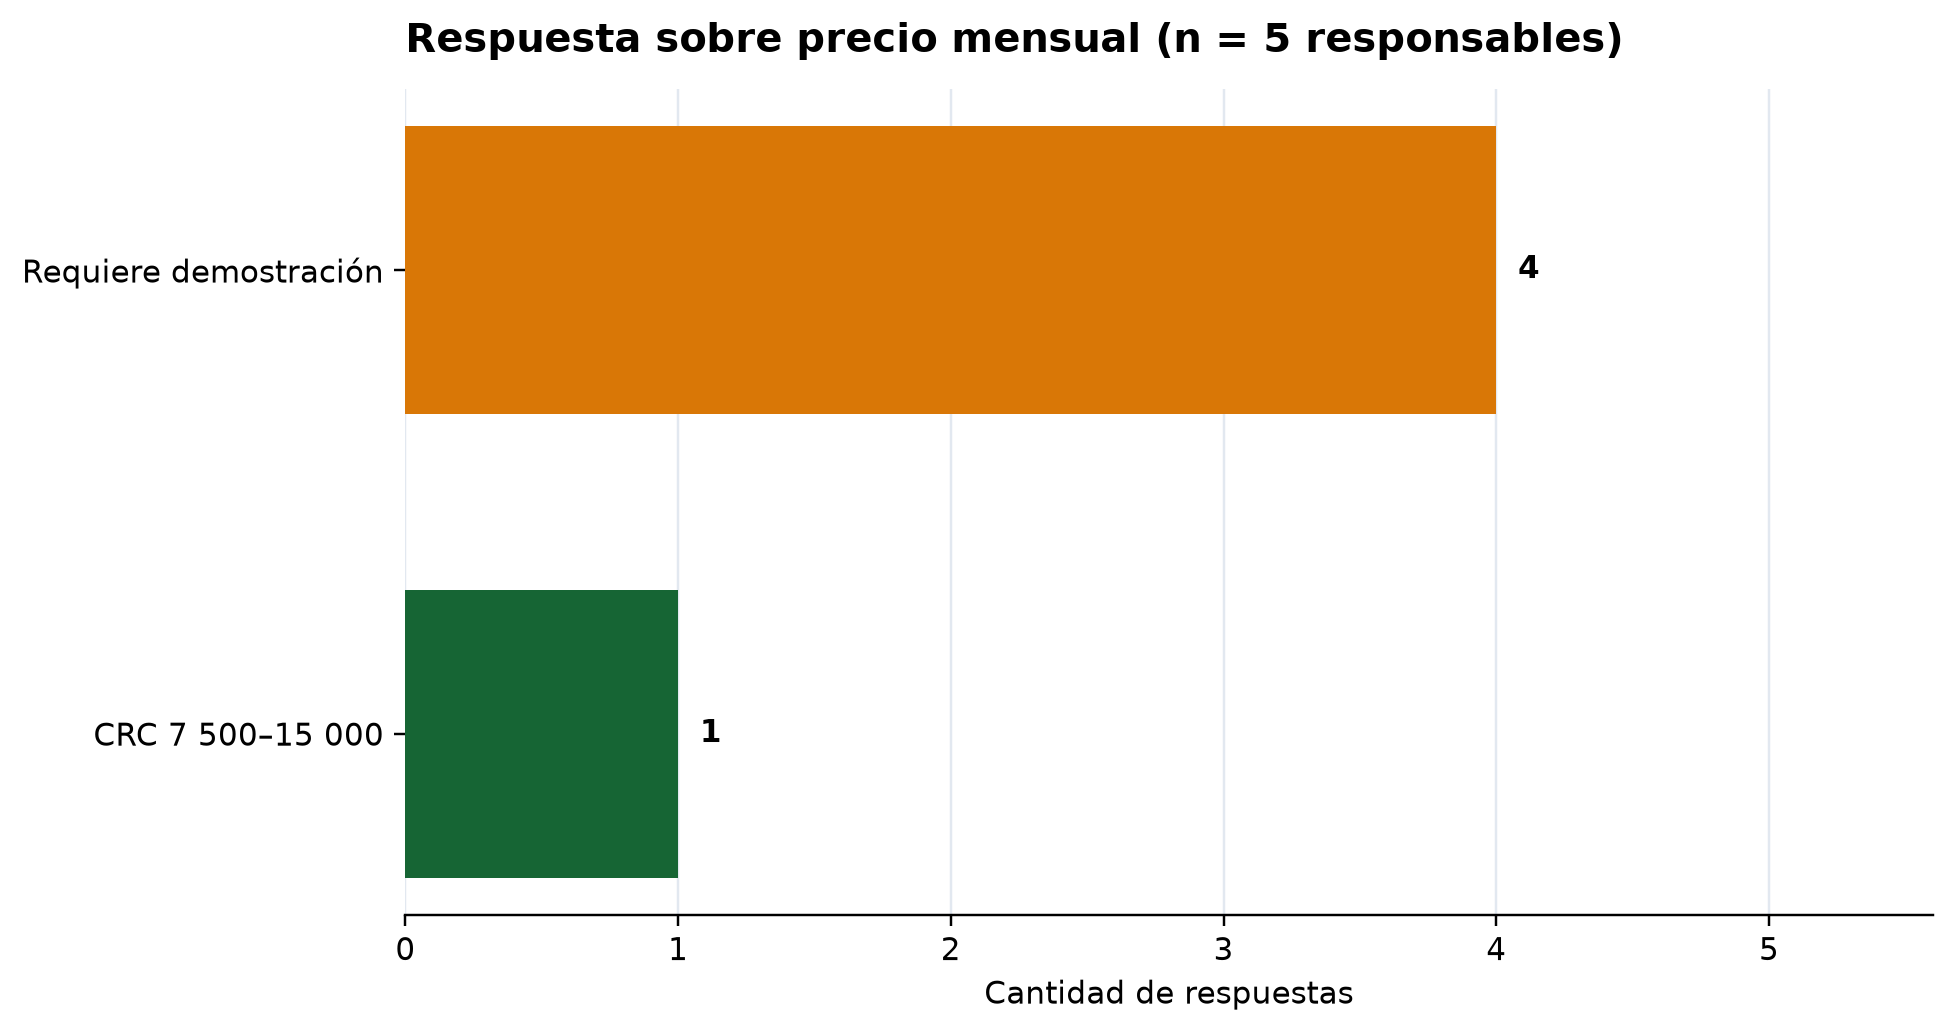
\includegraphics[width=0.86\textwidth]{imagenes/encuesta_disposicion_pago.png}
\caption{Respuesta de responsables sobre el precio mensual}
\label{fig:encuesta-precio}
\caption*{\textit{Nota}. Elaboración propia a partir de cinco respuestas administrativas \parencite{encuesta_gymhub_2026}.}
\end{figure}

\subsection{Resultados de miembros}

Siete miembros indicaron asistir tres o cuatro veces por semana y tres asisten
una o dos veces. Nueve señalaron que actualmente no consultan información del
gimnasio en formato digital. Nueve usarían Pulso principalmente desde el celular
y uno desde computadora. Nueve calificaron con 5 la utilidad de reunir pagos,
asistencia, rutina y progreso; uno la calificó con 4.

Entre las selecciones registradas, recordar vencimientos obtuvo seis menciones,
progreso cinco y encontrar la rutina tres. Los comentarios abiertos destacaron
rapidez, mantenimiento, actualización de rutinas, registro de pesos y acceso
centralizado. Estas respuestas orientan el diseño hacia la consulta de rutinas,
progreso y recordatorios desde el celular. Su uso se medirá durante el piloto.

\begin{figure}[htbp]
\centering
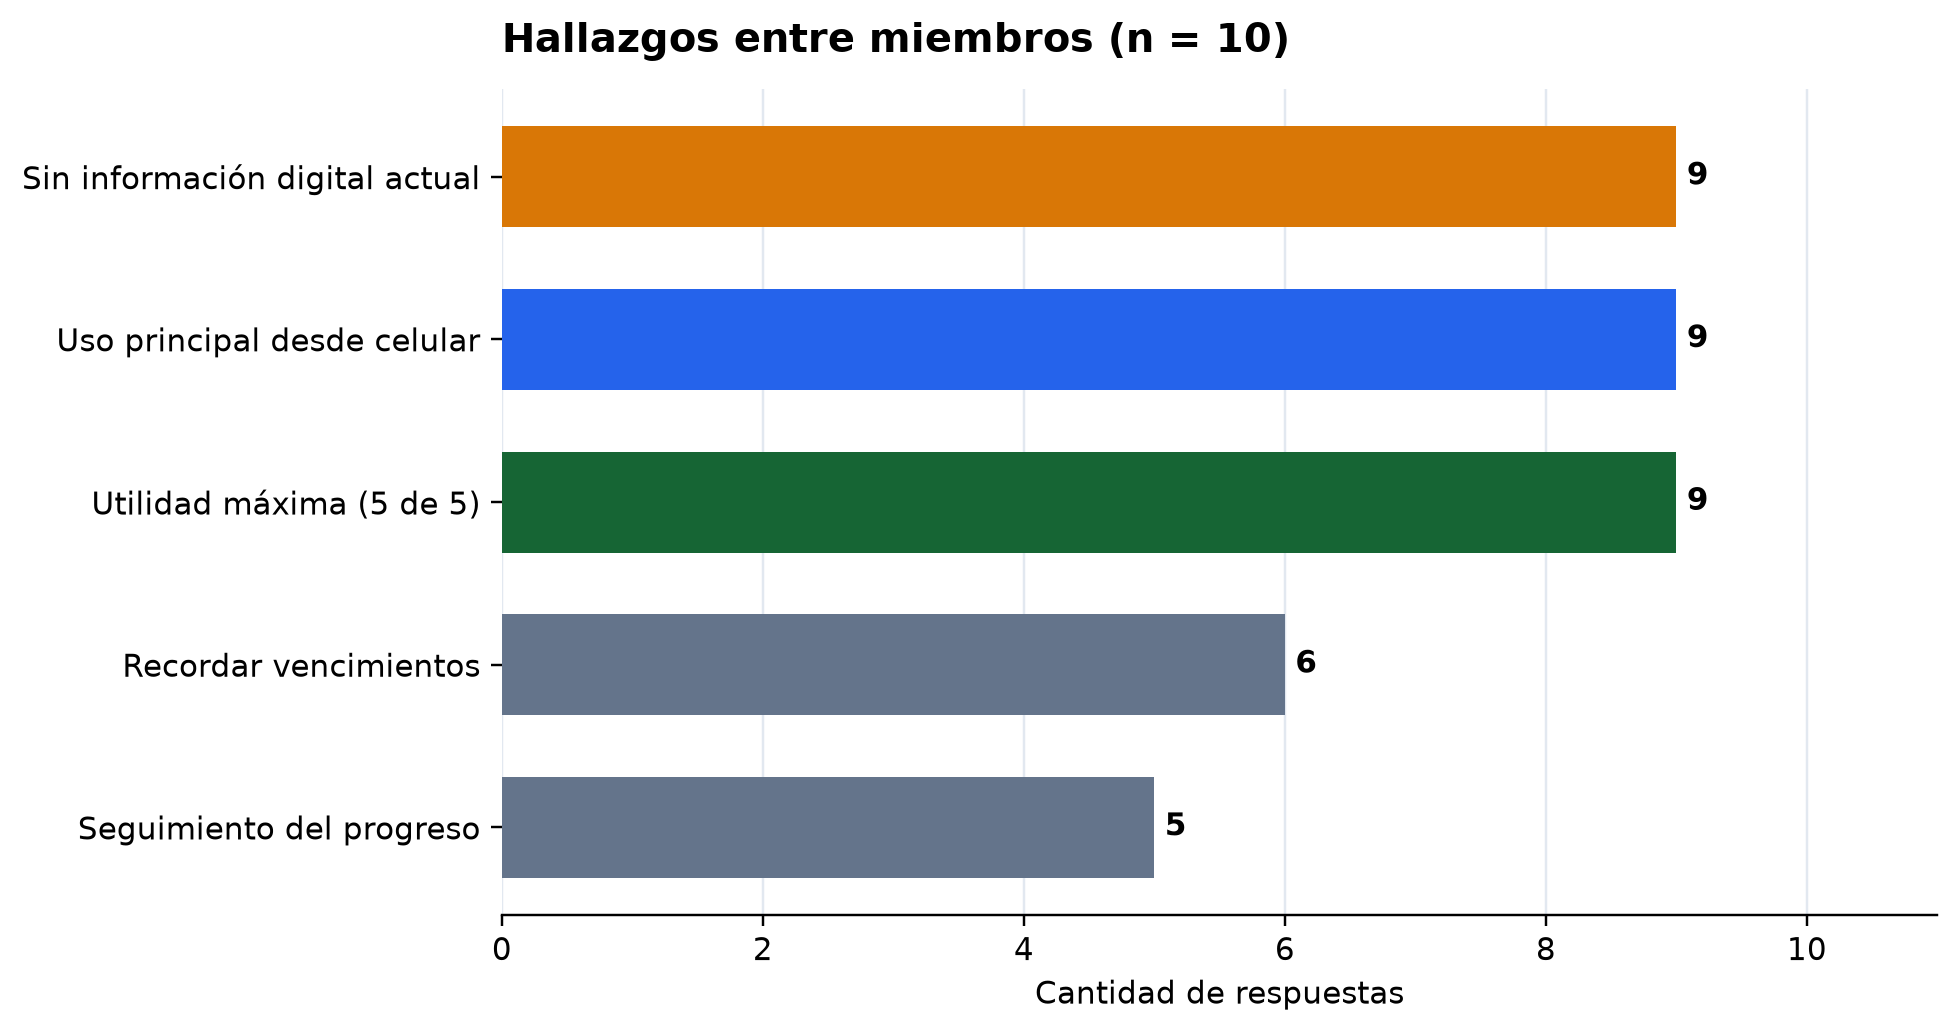
\includegraphics[width=0.9\textwidth]{imagenes/encuesta_resultados_miembros.png}
\caption{Hallazgos de miembros de gimnasios}
\label{fig:encuesta-miembros}
\caption*{\textit{Nota}. Al tratarse de preguntas de selección múltiple, las cantidades no corresponden a categorías excluyentes. Elaboración propia a partir de la encuesta \parencite{encuesta_gymhub_2026}.}
\end{figure}

\subsection{Alcance de los resultados}

Los resultados describen a las 15 personas participantes y no representan por sí
solos a todos los gimnasios de Pérez Zeledón. Aun con este alcance, permiten
tomar decisiones útiles: demostrar primero el control de cobros, priorizar el
acceso móvil, ofrecer una tarifa piloto y medir la continuidad después del uso.
El detalle metodológico y las diferencias entre el formulario previsto y el
aplicado se conservan en los apéndices.

Todavía falta información para estimar cuántos gimnasios del cantón podrían
contratar el servicio. La siguiente etapa registrará contactos, demostraciones,
rechazos y contrataciones. Pérez Zeledón será el punto de partida, con la
posibilidad de atender otros lugares mediante la plataforma web.

\subsection{Diseño del piloto}

Pit Bull Gym, ubicado en Mollejones, es el gimnasio aliado de Pulso para su
validación inicial. Su administración mostró interés en probar la aplicación y
valoró positivamente su potencial. El piloto aún no ha comenzado y se coordinará
con el gimnasio, de acuerdo con las condiciones de seguridad y responsabilidades
acordadas. Durante la capacitación se utilizarán datos ficticios; los datos
reales se incorporarán únicamente después de definir el consentimiento y los
procedimientos correspondientes.

Las respuestas anónimas de la encuesta son independientes de esta alianza.

\begin{table}[htbp]
\caption{Indicadores propuestos para un piloto}
\begin{tabularx}{\textwidth}{>{\bfseries}p{4cm}X p{3cm}}
\toprule
Indicador & Método & Meta inicial \\
\midrule
Activación & Responsables que completan configuración. & Definir con aliado. \\
Uso semanal & Sesiones activas por rol. & Establecer línea base. \\
Tareas completadas & Pagos, membresías y asistencias registradas. & Comparar con proceso previo. \\
Incidencias & Errores o dudas por semana. & Tendencia descendente. \\
Tiempo administrativo & Minutos para tareas seleccionadas. & Medir antes y después. \\
Continuidad & Intención de seguir y pagar. & Validar al cierre. \\
\bottomrule
\end{tabularx}
\caption*{\fuentepropia}
\end{table}

\subsection{Privacidad, imagen y propiedad intelectual}

La encuesta no solicitó nombres, correos ni datos de salud. Se limitó a personas
adultas e informó su finalidad educativa, la participación voluntaria y el uso
agregado de los resultados. Las capturas ocultan identificadores y utilizan
cuentas de demostración. Antes de operar con clientes se revisarán la base legal y
los procedimientos definitivos conforme a la Ley n.º 8968
\parencite{ley8968}.

Las imágenes incluidas son propias, licenciadas o citadas. No se utilizan logos de
gimnasios, personas identificables ni material de terceros sin permiso. El Canvas
se acredita como elaboración del equipo.

\subsection{Declaración del estado del proyecto}

Pulso nació como una idea propia en Fundamentos de Programación durante el
segundo periodo de 2025. En 2026 se amplió la primera versión y se preparó para
su primera participación en ExpoTÉCNICA. Por no haberse presentado en una
edición anterior, se inscribe como proyecto nuevo y no como proyecto de
continuación. Se cuenta con un MVP funcional, una demostración web y Pit Bull
Gym como aliado para la prueba inicial. El piloto aún no se ha ejecutado y sus
resultados de uso y continuidad comercial están pendientes de validación.
